\documentclass[a1paper, portrait, margin=0mm, innermargin=15mm,blockverticalspace=15mm, colspace=15mm, subcolspace=8mm]{tikzposter} 
	\usepackage{graphicx}
	\usepackage{subcaption}
	\usepackage{pgfplots}
	\usepackage{caption}
	\usepackage{natbib}
	\usepackage{hyperref}

    \title{Attacking Microcontrollers} 
    \institute{Schoold of Electronics and Computer Science, University of Southampton}
    \author{Author: Dionisio Perez-Mavrogenis (dpm3g10)\\
			Supervisor: Klaus-Peter Zauner (kpz)}
    \usetheme{Board} %Board is also cool

    
\definebackgroundstyle{die_image}{
\includegraphics[height=\paperheight, width=\paperwidth]{opt.jpg}
}
\usebackgroundstyle{Rays}    
    
\begin{document}

	\maketitle     
    \begin{columns} % See Section 4.4
        \column{0.5} % See Section 4.4
            \block{Microcontroller Introduction}{
                Microcontrollers can be found anywhere, from your cars stereo to missile launch panels and are usually cheap (around \pounds 2) and packed with information! They often come with crypto-engines (AES, DES and RSA are common) and hold all sorts of information like private crypto-keys for authentication or propietary algorithm implementations in the firmware or hardware, interesting all sorts of people into the contents of a microcontroller.
            } \qquad
            \block{Packaging and De-packaging}{
				Typically microcontrollers are too small and fragile to use as they are fabricated (with fabrication lengths shrank to micro-meters) and so they are packaged\citep{hwre}. Packacking material ranges depending on the microcontroller and its intended use,  but is usually hard epoxy resin \citep{sergei:thesis} \citep{hwre}. The packaging tries to protect the microcontroller from its external environment (humidity, radiation, temperature, crashes etc.) and also from prying eyes. Military-grade chips come with a lot of additional circuitry on the packaging whose responsibility is to detect tampering and respond in a suitable manner (even self destruction!) \citep{hwre}.\\
               De-packaging is not always requierd and the methods depend on the packaging used and protective mechanisms in place, but on epoxy-packaged chips one can etch the epoxy away by using HNO$_3$ or H$_2$SO$_4$ and then cleaning the chip in an ultrasonic bath \citep{sergei:thesis} \citep{hwre}. For other packaging types, e.g. metal, ceramic or plastic, one can use similar techniques and tools, e.g. drills or a blowtorch \citep{hwre}.De-packaging is usually easier than expected and removing simple epoxy resin can be done with readily available chemicals \citep{hwre}. Fig.~\ref{328c} and Fig.~{328o} show a microcontroller in its factory resin packaging and the exposed die after chemical decapsulation\citep{siliconpr0n_328}.
               		
	
		\begin{minipage}{0.5\linewidth}
			\begin{tikzfigure}[ATmega328 with epoxy resin packaging.]
				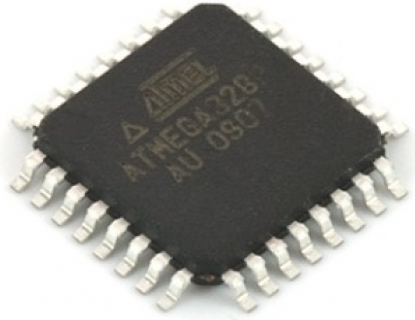
\includegraphics[width=0.7\textwidth]{atmega328.jpg}
				\label{328c}
			\end{tikzfigure}
		\end{minipage}% <--- the percent character will "comment out" the new line    
		\begin{minipage}{0.5\linewidth}
			\begin{tikzfigure}[The exposed die of an ATmega328.]
				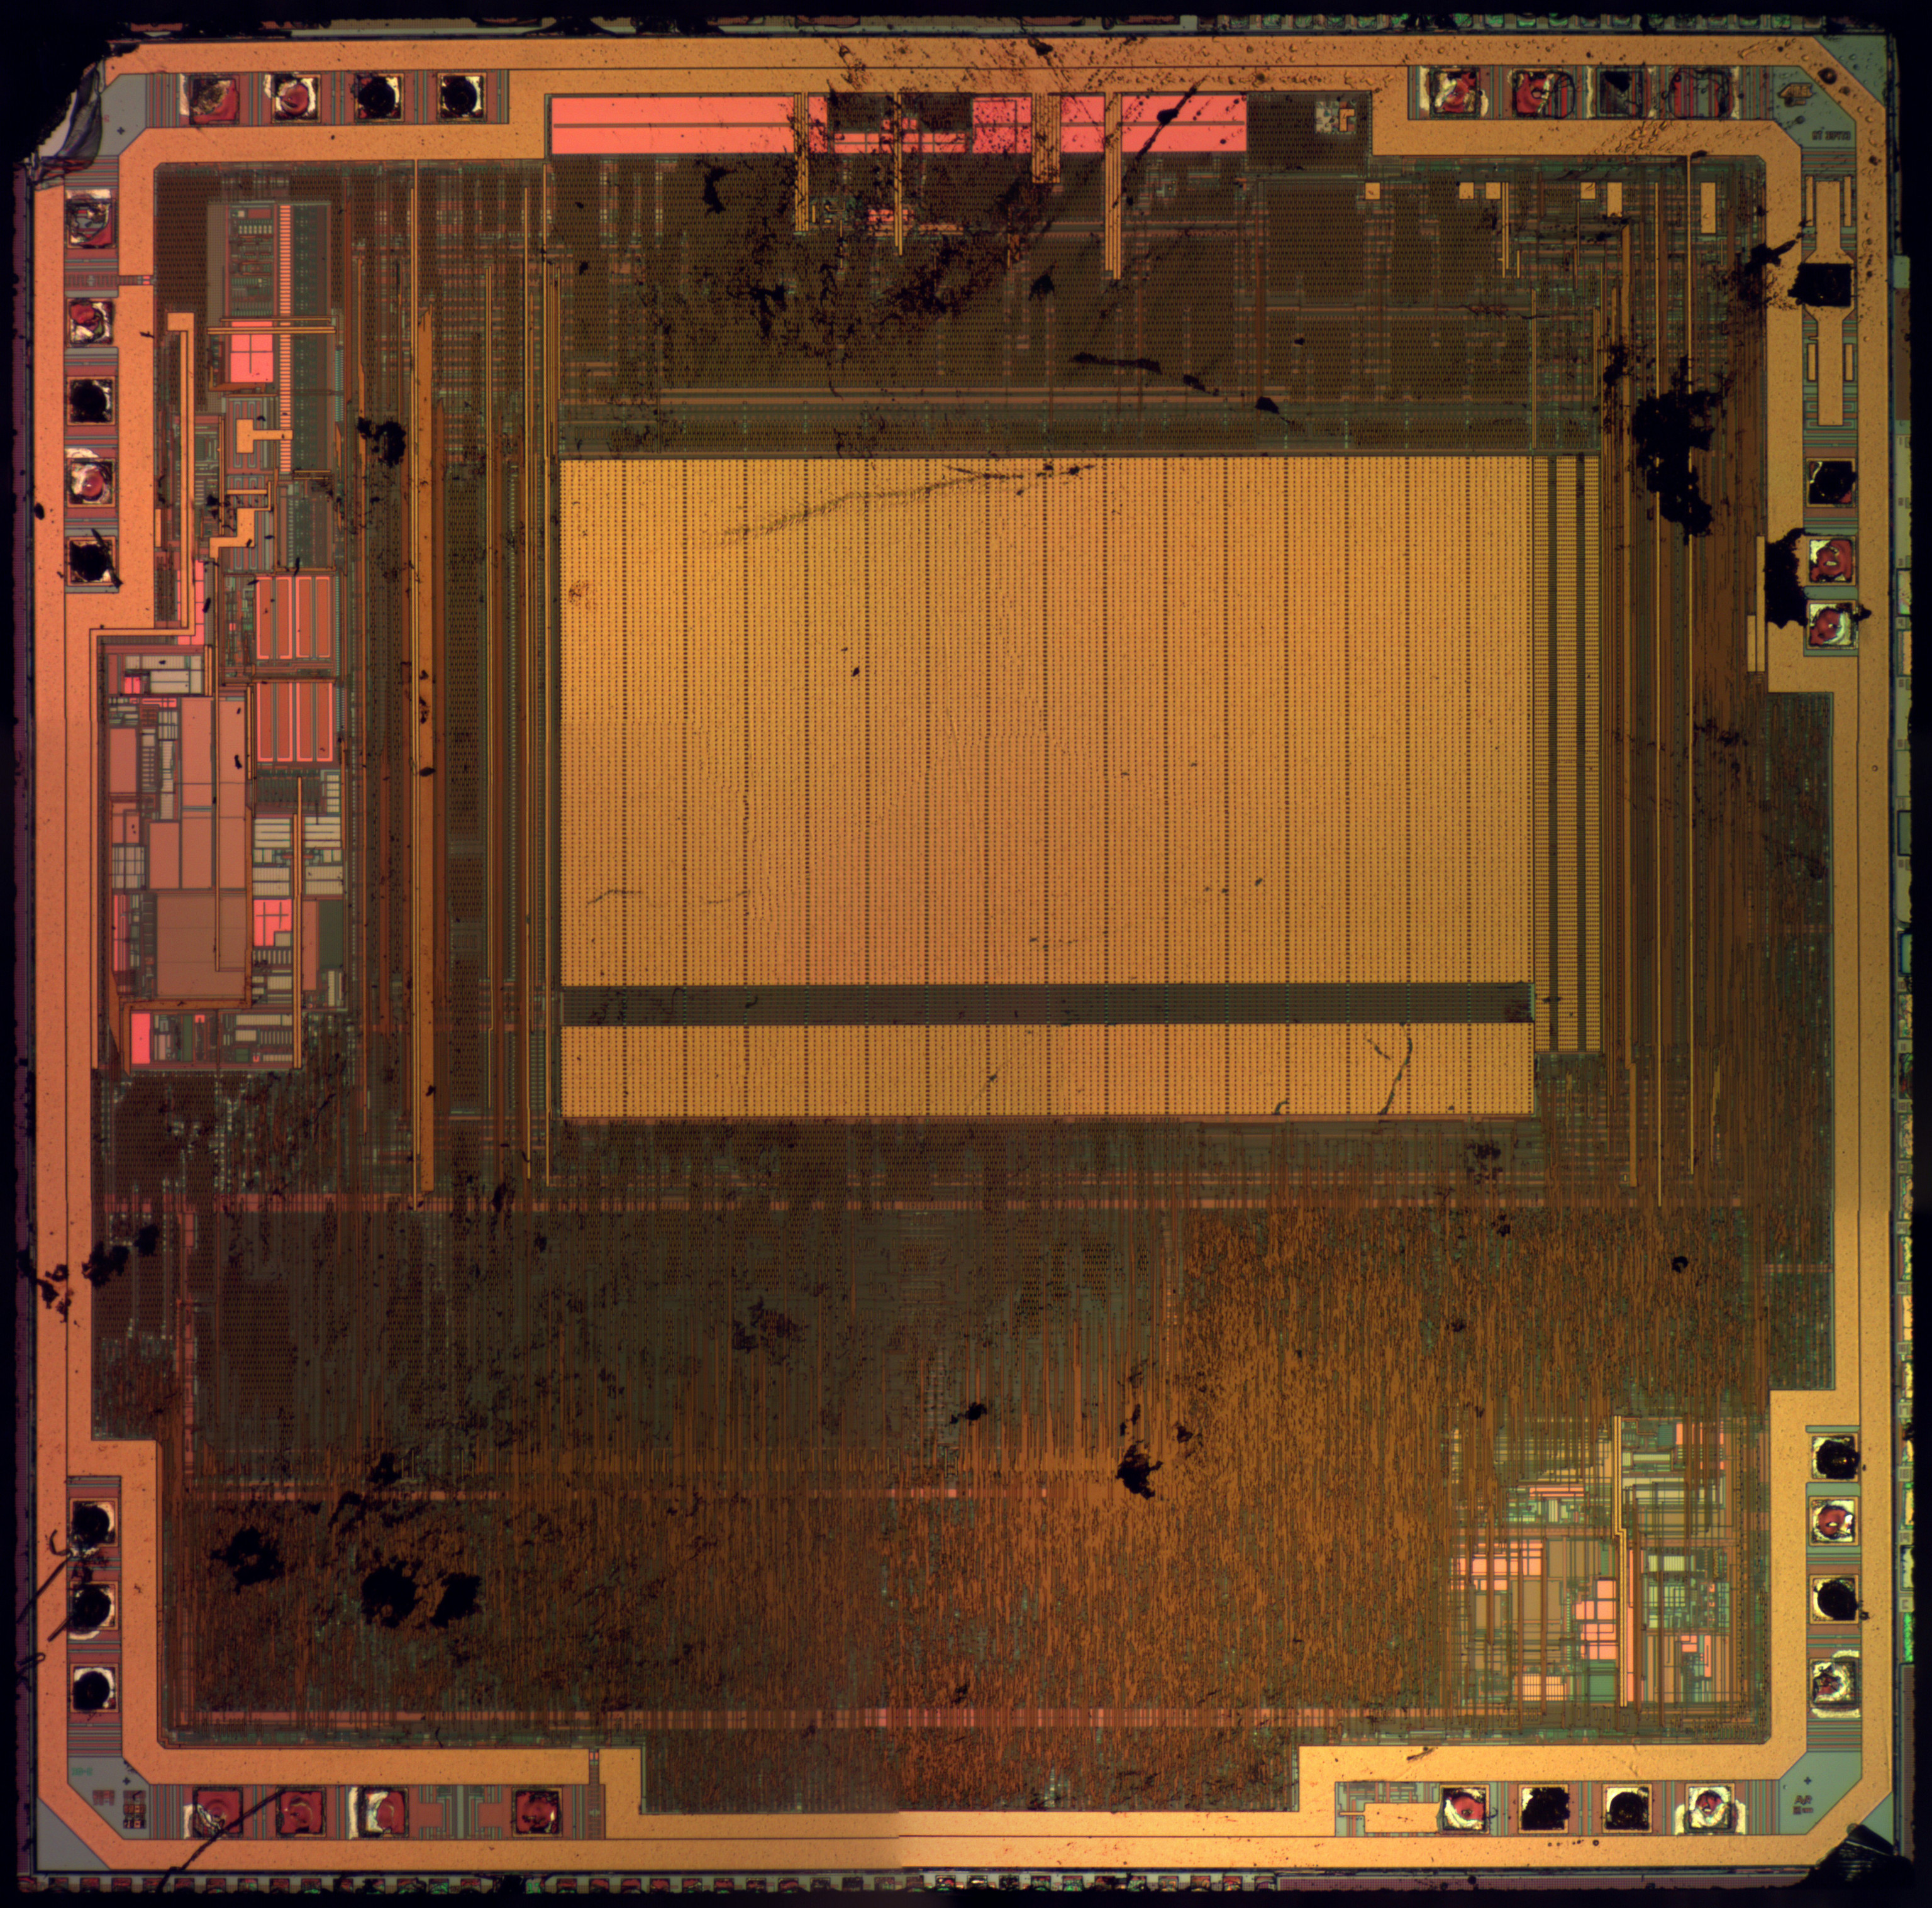
\includegraphics[width=0.7\textwidth]{atmega328_open.jpg}
				\label{328o}
			\end{tikzfigure}
		\end{minipage}
               
          }% end block

            \note[rotate=15, width=15cm, targetoffsetx=5cm,targetoffsety=-5cm]{tampering detection means detecting abnormalities in voltage, clock frequency, radiation, tilting etc.}
                
        \column{0.5}
        	\block{Attack Types}{
				\textbf{Non-invasive} attacks are cheap and easy to perform and require no decapsulation. Popular methods include are power analysis and fault injection, where faults may be injected by exposing the chip to environmental conditions that it was not meant to work in.
				
				
			Fig.~\ref{concept} describes the relative diffuclty of the attacks methods (green) and complexity of the defensive mechanisms (red), where the notions of difficulty and complexity incorporate the skill, money and machinery needed.			
				
				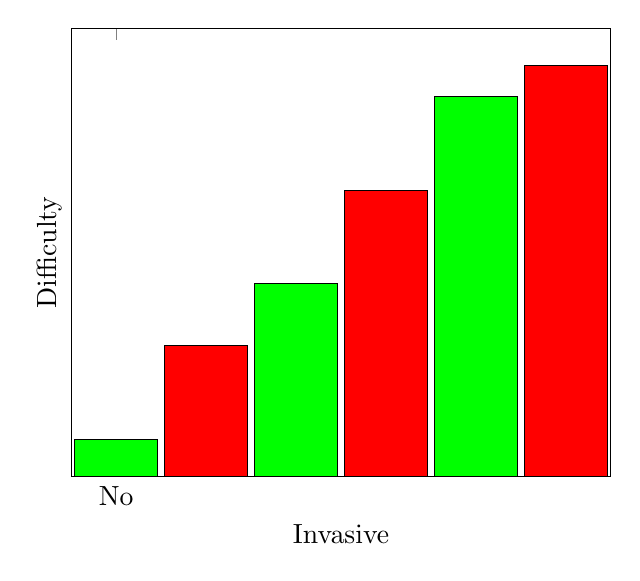
\begin{tikzpicture}{Relative difficulties of attack and defensive mechanisms.}
				\label{concept}
						\begin{axis}[ytick=\empty, bar width=30pt,symbolic x coords={No, no, Semi,semi, Full,full},xtick=data, ylabel = Difficulty,xlabel = Invasive]
			        	    \addplot[ybar,fill=green] coordinates {
    	    		    	    (No, 35)
				            };		
    	    			    \addplot[ybar, fill=red]coordinates{
        				    	(no, 50)
		    	        	};
		    	        	\addplot[ybar,fill=green] coordinates {
    	    		    	    (Semi, 60)
				            };		
    	    			    \addplot[ybar, fill=red]coordinates{
        				    	(semi, 75)
		    	        	};
		    	        	\addplot[ybar,fill=green] coordinates {
    	    		    	    (Full, 90)
				            };		
    	    			    \addplot[ybar, fill=red]coordinates{
        				    	(full, 95)
		    	        	};
			    	    \end{axis}		
					\end{tikzpicture}
				attacks require decapsulation and are a lot more technical, expensive (to perform and repliate) and time consuming with manufacturer-equivalent machinery used. 
        	}
            \block{Sample Attack}{
                provide atmega644 characteristics.
                set attack scenario, type, setup and exact details
            }
    \end{columns}
    
\bibliographystyle{plain}
    
    \block[roundedcorners=65]{}{{\tiny \bibliography{poster}}}
\end{document}